% !TEX root = saveliev_physics_general_course_1.tex
%!TEX TS-program = pdflatex
%!TEX encoding = UTF-8 Unicode

\chapter[NHỮNG SỰ CÂN BẰNG VÀ BIẾN ĐỔI PHA]{NHỮNG SỰ CÂN BẰNG\\ VÀ BIẾN ĐỔI PHA}\label{chap:15}
\chaptermark{NHỮNG SỰ CÂN BẰNG PHA VÀ BIẾN ĐỔI PHA}

\section{Mở đầu}\label{sec:15_1}
%By a phase in thermodynamics is meant a combination of homogeneous parts of a system having identical properties. Let us explain what is meant by this definition using the following examples. A closed vessel contains water and a mixture of air and water vapour above it. Here we have to do with a system consisting of two phases: one is formed by the water, and the other by the mixture of air and water vapour. If we add a few pieces of ice to the water, then all these pieces form a third phase. Different crystalline modifications of a substance are also different phases. For instance, diamond and graphite are different solid phases of carbon.
Trong nhiệt động học ta gọi pha là một tập hợp các phần đồng tính, có tính chất như nhau của một hệ thống. Ta hãy nói rõ khái niệm pha bằng những ví dụ sau đây. Trong một bình kín có nước và trên đó có hỗn hợp không khí và hơi nước. Trong trường hợp này, ta có một hệ gồm hai pha: một pha là nước và pha thứ hai là hỗn hợp không khí và hơi nước. Nếu ta thêm vào nước một vài mẩu nước đá thì những mẩu nước đá này tạo thành pha thứ ba. Những hình thức kết tinh khác nhau của bất kỳ chất nào cũng là những pha khác nhau. Chẳng hạn như kim cương và graphite là những pha rắn khác nhau của cacbon.\\

%In definite conditions, different phases of the same substance can be in equilibrium with one another while being in contact. The equilibrium of two phases is possible only within a definite temperature interval, and a quite definite pressure $p$ at which equilibrium is possible corresponds to each value of the temperature $T$. Thus, the equilibrium states of two phases will be depicted in a $p$-$T$ diagram by the line
Trong những điều kiện xác định, những pha khác nhau của cùng một chất có thể đứng cân bằng với nhau, trong khi vẫn tiếp xúc với nhau. Sự cân bằng của hai pha chỉ có thể có được trong một khoảng nhiệt độ xác định; khi đó, mỗi giá trị của nhiệt độ $T$ ứng với một áp suất $p$ hoàn toàn xác định trong đó có thể có trạng thái cân bằng. Vì vậy, những trạng thái cân bằng của hai pha được biểu diễn trên giản đồ ($p,T$) bằng đường
\begin{equation}\label{eq:15_1}
    p = f(T)
\end{equation}

%Three phases of a single substance (solid, liquid, and gaseous, or liquid and two solid phases) can be in equilibrium only at single values of the temperature and pressure which in the $p$-$T$ diagram correspond to what we call the \textbf{triple point}. This point is at the intersection of the equilibrium curves for the phases taken in pairs.
Ba pha của cùng một chất (rắn, lỏng và khí hoặc lỏng và hai pha rắn) chỉ có thể đứng cân bằng với nhau ở một giá trị duy nhất của nhiệt độ và áp suất; trên giản đồ ($p,T$) các giá trị này ứng bới một điểm là \textbf{điểm ba}. Điểm này nằm tại giao điểm của các đường cong cân bằng pha, lấy từng cặp một.\\

%It is proved in thermodynamics, in agreement with experiments, that the equilibrium of more than three phases of the same substance is impossible.
Trong nhiệt động học người ta đã chứng minh là không thể nào có được sự cân bằng của nhiều hơn ba pha của cùng một chất; điều này cũng phù hợp với thực nghiệm.\\

%The transition from one phase to another is usually attended by the absorption or liberation of a certain amount of heat called the \textbf{latent heat of transition} or simply the \textbf{heat of transition}. Such transitions are called phase transitions of the first kind. There are also transitions from the crystalline modification to another that are not associated with the absorption or liberation of heat. These transitions are called phase transitions of the second kind\footnote{Phase transitions of the second kind do not exhaust the transitions between different crystalline modifications. They include the transition to a superconductive state performed in the absence of a magnetic field, and also the transition between the two liquid phases of helium called helium-I and helium-II.}. We shall consider only transitions of the first kind.
Việc chuyển từ một pha sang một pha khác thường kèm theo sự hấp thụ hoăc sự tỏa một nhiệt lượng nào đó mà người ta gọi là \textbf{ẩn nhiệt của sự chuyển}, hoặc đơn giản là \textbf{nhiệt của sự chuyển}. Những sự chuyển như vậy gọi là những sự chuyển pha loại một. Còn có những sự chuyển pha từ hình thức kết tinh này sang hình thức kết tinh khác. Những sự chuyển này không gắn với sự hấp thụ hoặc tỏa nhiệt lượng. Những sự chuyển pha loại đó gọi là những sự chuyển pha loại hai\footnote{Những sự chuyển pha loại hai không chỉ bao gồm những sự chuyển giữa các hình thức kết tinh khác nhau. Trong số chuyển pha loại hai còn có sự chuyển sang trạng thái siêu dẫn được thực hiện khi không có từ trường và cả sự chuyển giữa hai pha lỏng của heli là heli I và heli II.}. Chúng ta chỉ hạn chế trong việc xét những sự chuyển pha loại một.\\

\section{Sự bay hơi và sự ngưng tụ}\label{sec:15_2}

%Liquids and solids at any temperature contain a certain number of molecules whose energy is sufficient for them to overcome the attraction to other molecules, escape from the surface of the liquid or solid and to pass over into the gaseous phase. The transition of a liquid into the gaseous phase is called \textbf{vaporization} or \textbf{evaporation}, and the transition of a solid into the gaseous phase is called \textbf{sublimation}.
Trong các chất lỏng và các chất rắn ở bất kỳ nhiệt độ nào cũng có một số phân tử có năng lượng đủ lớn để có thể thắng được lực hút của các phân tử khác và rời bỏ chất lỏng hoặc chất rắn và đi vào pha khí. Sự chuyển của chất lỏng thành trạng thái khí gọi là \textbf{sự bay hơi}, sự chuyển của chất rắn sang trạng thái khí gọi là \textbf{sự thăng hoa}.\\

%All solids sublime to some extent without any exception. In some substances such as carbon dioxide, sublimation proceeds at an appreciable rate; in other substances, it is so insignificant at ordinary temperatures that it is practically not detected.
Tất cả các vật rắn, không có trường hợp nào ngoại lệ cả, đều bị thăng hoa ở mức độ này hay mức độ khác. Ở những chất này, chẳng hạn ở cacbonic, quá trình thăng hoa xảy ra với tốc độ đáng kể; ở những chất khác, ở những nhiệt độ thông thường, quá trình này xảy ra chậm đến nỗi ta hầu như không phát hiện ra được.\\

%In evaporation and sublimation, the fastest molecules leave a body. As a result, the mean energy of the remaining molecules diminishes, and the body cools. To maintain the temperature of an evaporating (or subliming) body at a constant value, heat must continuously be supplied to it. The heat $L$ that must be supplied to a unit mass of a substance to transform it into a vapour at the same temperature which the substance had prior to evaporation is defined as the \textbf{specific heat of vaporization} (or sublimation).
Khi bay hơi và khi thăng hoa những phân tử chuyển động nhanh nhất rời khỏi vật, do đó năng lượng trung bình của các phân tử còn lại giảm đi và vật bị lạnh đi. Để giữ cho nhiệt độ của vật bị bay hơi (hay bị thăng hoa) không thay đổi thì phải liên tục cung cấp nhiệt lượng cho nó. Nhiệt lượng $L$ cần phải cung cấp cho một đơn vị khối lượng của một chất để biến nó thành hơi ở cùng nhiệt độ với vật trước khi bay hơi được gọi là \textbf{nhiệt bay hơi} (hoặc thăng hoa).\\

%In condensation, the heat for evaporation is returned: the liquid (or solid) formed upon condensation is heated.
Khi ngưng tụ thì nhiệt lượng bị mất, khi bay hơi sẽ được trả trở lại: chất lỏng (hoặc chất rắn) được tạo thành khi ngưng tụ bị nóng lên.\\

%Let us consider the setting in of equilibrium between a liquid and its vapour. We shall take a sealed vessel partly filled with a liquid (\fig{15_1}) and assume that initially the substance was completely removed from the space above the liquid. Owing to evaporation, the space above the liquid will become filled with molecules. The molecules that passed into the gaseous phase move chaotically and collide with the surface of the liquid. Some of these collisions will be attended by transition of the molecules into the liquid phase. The number of molecules passing in unit time into the liquid phase is evidently proportional to the number of molecules colliding with its surface. This number, in turn, is proportional to $n\average{v}$ [see \eqn{11_23}], \ie, grows with increasing pressure $p$. Hence, evaporation is accompanied by the reverse process of transition of the molecules from the gaseous to the liquid phase, its intensity growing as the density of the molecules in the space over the liquid increases. When a certain quite definite (for the given temperature) pressure is reached, the number of molecules escaping from the liquid will become equal to that returning to it. Beginning from this moment, the density of the vapour stops changing. Mobile equilibrium sets in between the liquid and its vapour, and it will exist until the volume or the temperature of the system changes. A vapour in equilibrium with its liquid is called \textbf{saturated}. The pressure at which equilibrium is observed is called the \textbf{saturated vapour pressure}.
Ta hãy xét quá trình thiết lập sự cân bằng giữa chất lỏng và hơi của nó. Ta lấy một bình kín chứa một phần chất lỏng (\fig{15_1}) và giả sử ban đầu tất cả các chất ở trong không gian nằm trên chất lỏng đã được lấy đi hết. Do quá trình bay hơi, khoảng không gian nằm trên chất lỏng sẽ chứa đầy những phân tử. Những phân tử, sau khi chuyển sang pha khí, sẽ chuyển động hỗn loạn, va chạm với mặt ngoài của chất lỏng; đồng thời một phần của những va chạm đó sẽ kèm theo với sự chuyển của các phân tử sang pha lỏng. 
\begin{figure}[!h]
	\begin{center}
		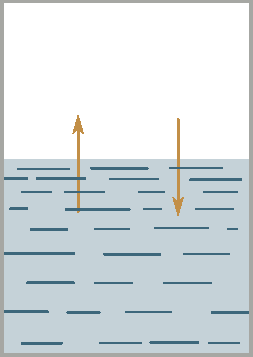
\includegraphics[scale=0.9]{figures/ch_15/fig_15_1.pdf}
		\caption[]{}
		\label{fig:15_1}
	\end{center}
	\vspace{-0.8cm}
\end{figure}
Số lượng phân tử được chuyển trong đơn vị thời gian sang pha lỏng dĩ nhiên tỷ lệ với số phân tử va chạm vào mặt ngoài; số phân tử này lại tỷ lệ với $n\average{v}$ (xem \eqn{11_23}), tức là tăng với áp suất $p$. Do đó, song song với quá trình bay hơi diễn ra một quá trình ngược lại trong đó các phân tử chuyển từ pha khí sang pha lỏng; đồng thời cường độ của quá trình này tăng khi mật độ phân tử trong vùng không gian trên chất lỏng tăng lên.Khi đạt tới một áp suất hoàn toàn xác định nào đó (ở nhiệt độ đã cho) thì số phân tử rời khỏi chất lỏng và số phân tử quay trở lại chất lỏng sẽ trở nên bằng nhau. Từ lúc đó trở đi, mật độ của hơi sẽ không thay đổi nữa. Giữa chất lỏng và hơi hình thành một sự cân bằng động, cân bằng này tồn tại mãi nếu thể tích hoặc nhiệt độ của hệ không bị thay đổi. Chất hơi nằm cân bằng với chất lỏng của nó gọi là \textbf{hơi bão hòa}. Áp suất tại đó quan sát thấy sự cân bằng gọi là \textbf{áp suất hơi bão hòa}.\\



%The number of molecules leaving a liquid in unit time grows very rapidly with the temperature. The number of molecules colliding with the surface of the liquid depends on the temperature to a smaller extent (through $\average{v}$ in proportion to $\sqrt{T}$). Therefore, upon elevation of the temperature, equilibrium between the phases is violated, and during a certain time the stream of molecules travelling in the direction liquid $\to$ vapour will exceed their stream in the direction vapour $\to$ liquid. This continues until the increase in the pressure again leads to the setting in of mobile equilibrium. Thus, the pressure at which mobile equilibrium sets in between a liquid and its vapour, \ie, the saturated vapour pressure, is found to depend on the temperature. The form of this relation is shown in \fig{15_2}. The meaning of the symbols $\ab{T}{cr}$ and $\ab{p}{cr}$ will come to light in \sect{15_4}.
Số phân tử rời bỏ chất lỏng trong một đơn vị thời gian tăng rất mạnh theo nhiệt độ. Số phân tử va chạm với mặt chất lỏng phụ thuộc vào nhiệt độ ở cấp thấp hơn (tính thông qua $\average{v}$ như $\sqrt{T}$). Vì vậy, khi tăng nhiệt độ, sự cân bằng giữa các pha bị phá huỷ, và trong một khoảng thời gian nào đó dòng phân tử đi theo hướng chất lỏng $\to$ hơi sẽ lớn hơn dòng phân tử đi theo hướng hơi $\to$ chất lỏng. Sự kiện này kéo dài cho đến khi sự tăng của áp suất lại dẫn tới việc thiết lập trạng thái cân bằng động. Vì vậy áp suất trong đó sự cân bằng động giữa chất lỏng và hơi đuọc thiết lập, tức là áp suất hơi bão hòa, phụ thuộc vào nhiệt độ. Dạng của sự phụ thuộc đó được vẽ trên \fig{15_2}. Ý nghĩa của các ký hiệu $\ab{T}{th}$ và $\ab{p}{th}$ sẽ được giải thích rõ ở \sect{15_4}; $\ab{T}{b}$ là điểm ba (\sect{15_8}).

\begin{figure}[!htb]
	\begin{center}
		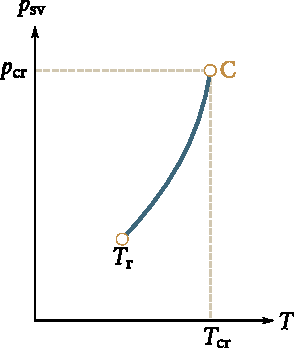
\includegraphics[scale=0.95]{figures/ch_15/fig_15_2.pdf}
		\caption[]{}
		\label{fig:15_2}
	\end{center}
	\vspace{-0.8cm}
\end{figure}

%If we increase the volume of the vessel, the vapour pressure will drop, and equilibrium will be violated. As a result, an additional amount of the liquid will transform into a vapour to make the pressure equal to $\ab{p}{sv}$, again. Similarly, reduction of the volume will cause a certain amount of the vapour to transform into a liquid.
Nếu tăng thể tích của bình chứa, áp suất hơi sẽ giảm và cân bằng sẽ bị phá huỷ. Kết quả là một lượng chất lỏng bổ sung sẽ bị biến thành hơi, sao cho áp suất lại trở nên bằng $\ab{p}{th}$. Tương tự như vậy, việc giảm thể tích sẽ dẫn tới việc biến đổi một lượng hơi nào đó thành chất lỏng.

%Everything said above about equilibrium between a liquid and a gas also holds for a solid-gas system. A definite value of the pressure at which mobile equilibrium sets in between the solid and the gas corresponds to every temperature. For many bodies such as solid metals, this pressure at ordinary temperatures is so small that it cannot be detected by the most sensitive instruments.
Tất cả những điều nói về sự cân bằng giữa chất lỏng và chất khí cũng đúng đối với hệ chất rắn - khí. Mỗi nhiệt độ ứng với một giá trị xác định của áp suất trong đó thiết lập sự cân bằng động giữa chất rắn và chất khí. Đối với nhiều vật, chẳng hạn đối với các kim loại rắn, ở những nhiệt độ thông thường áp suất đó nhỏ đến nỗi không thể phát hiện được ngay cả với những dụng cụ nhạy nhất.

\section{Sự cân bằng của chất lỏng\\ và hơi bão hòa}\label{sec:15_3}

%Let us consider the compression of a substance at a constant temperature. Assume that the substance is initially gaseous. First, the pressure of the gas will grow with decreasing volume (\fig{15_3}). When the volume $\ab{V}{g}$ is reached, the pressure stops changing, and the substance stops being homogeneous---part of the gas condenses into a liquid. The substance stratifies into two phases: a liquid and a gaseous one. A further reduction of the volume is attended by more and more of the substance passing over into the liquid phase, the transition occurring at a constant pressure $\ab{p}{sv}$ (the saturated vapour pressure). After condensation of the substance terminates (this occurs when the volume $\ab{V}{lq}$ is reached), a further reduction in the volume begins to be attended by a rapid growth of the pressure.
Ta hãy xét quá trình nén một chất ở nhiệt độ không đổi. Giả thiết rằng ban đầu chất đó ở dạng khí. Thoạt đầu, khi giảm thể tích, áp suất chất khí sẽ tăng (\fig{15_3}). Khi đạt tới thể tích $\ab{V}{k}$ thì áp suất không thay đổi nữa, còn chất đó không còn là đồng tính nữa, nghĩa là một phần chất khí bị ngưng tụ thành chất lỏng. Sẽ xảy ra sự phân chất thành hai pha: lỏng và khí. Khi tiếp tục giảm thể tích, phần chất chuyển sang pha lỏng ngày càng lớn, đồng thời sự chuyển đó diễn ra ở áp suất không đổi $\ab{p}{bh}$ (áp suất hơi bão hòa). Sau khi quá trình ngưng tụ của chất chấm dứt (điều đó xảy ra khi thể tích đạt tới giá trị $\ab{V}{l}$), thì sự giảm tiếp tục của thể tích sẽ đi kèm theo sự tăng rất nhanh của áp suất.


\begin{figure}[!htb]
	\begin{center}
		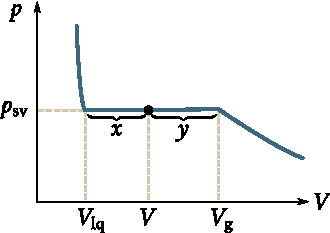
\includegraphics[scale=1]{figures/ch_15/fig_15_3.pdf}
		\caption[]{}
		\label{fig:15_3}
	\end{center}
	\vspace{-0.8cm}
\end{figure}

%In \fig{15_3}, $\ab{V}{ab}$ is the volume occupied by the substance in the gaseous state at the pressure $\ab{p}{sv}$ and $\ab{V}{lq}$ is the volume of the substance in the liquid state at the same pressure. At any intermediate value of the volume $V$, part of the substance with the mass $\ab{m}{lq}$ will be in the liquid state, and part with the mass $\ab{m}{v}$ in the vapour state. Let us find the ratio $\ab{m}{lq}/\ab{m}{v}$.
Trên \fig{15_3}, $\ab{V}{k}$ là thể tích của chất đó ở trạng thái khí dưới áp suất $\ab{p}{bh}$, $\ab{V}{l}$ là thể tích của chất đó ở trạng thái lỏng và cũng dưới áp suất đó. Ở bất kỳ giá trị trung gian nào của thể tích $V$ cũng có một phần khối lượng $\ab{m}{l}$ của chất đó ở trạng thái lỏng và một phần có khối lượng $\ab{m}{k}$ ở trạng thái hơi. Ta hãy tìm tỉ số $\ab{m}{l}/\ab{m}{k}$.\\ 

%We shall call the volume of a unit mass of a substance its specific volume $V'$. Thus, if the mass of a substance is $m$, then the specific volumes of its saturated vapour and liquid at the pressure $\ab{p}{sv}$ will be
Ta gọi thể tích riêng $V'$ là thể tích của đơn vị khối lượng của chất đó. Khi đó, nếu khối lượng của chất bằng $m$ thì thể tích riêng của hơi bão hòa và của chất lỏng dưới áp suất $\ab{p}{bh}$ sẽ bằng

\begin{equation}\label{eq:15_2}
    \ab{V}{h}' = \frac{\ab{V}{k}}{m},\quad \ab{V}{l}' = \frac{\ab{V}{l}}{m}.
\end{equation}

\noindent
%In the state when the mass of the liquid phase is $\ab{m}{lq}$ and that of the vapour is $\ab{m}{v}$, the liquid will occupy the volume $\ab{V}{lq}'\ab{m}{lq}$, and the saturated vapour, the volume $\ab{V}{v}'\ab{m}{v}$. The sum of these two volumes must equal the volume $V$:
Ở trạng thái mà khối lượng pha lỏng là $\ab{m}{l}$, còn khối lượng pha hơi là $\ab{m}{h}$ thì thể tích của phần chất lỏng sẽ là $\ab{V}{l}'\ab{m}{l}$ và thể tích của phần hơi bão hòa sẽ là $\ab{V}{h}'\ab{m}{h}$. Tổng của cả hai thể tích đó phải bằng thể tích $V$:
\begin{equation*}
    V = \ab{V}{l}'\ab{m}{l} + \ab{V}{h}'\ab{m}{h}.
\end{equation*}

\noindent
%Introducing into this equation expressions~\eqref{eq:15_2} for the specific volumes and substituting the $\ab{m}{lq}+\ab{m}{v}$ for the mass $m$, we get
Thế biểu thức \eqref{eq:15_2} đối với các thể tích riêng vào đó và thay khối lượng $m$ bằng tổng $\ab{m}{l} + \ab{m}{h}$, ta được:
\begin{equation*}
    V = \ab{V}{l}' \parenthesis{\frac{\ab{m}{l}}{\ab{m}{l}+\ab{m}{h}}} + \ab{V}{h}' \parenthesis{\frac{\ab{m}{h}}{\ab{m}{l}+\ab{m}{h}}}.
\end{equation*}

\noindent
%Hence,
Từ đây rút ra:
\begin{equation}\label{eq:15_3}
    \frac{\ab{m}{l}}{\ab{m}{h}} = \frac{\ab{V}{k} - V}{V - \ab{V}{l}} = \frac{y}{x}
\end{equation}

\noindent
%(see \fig{15_3}). Thus, the ratio of the masses of the liquid and the saturated vapour in a two-phase state equals the ratio of the lengths into which the point depicting the state divides the horizontal portion of the isotherm.
(Xem \fig{15_3}). Vì vậy, tỷ số khối lượng của chất lỏng và hơi bão hòa ở trạng thái hai pha sẽ bằng tỷ số của các đoạn thẳng mà điểm biểu diễn trạng thái đã chia trên đoạn nằm ngang của đường đẳng nhiệt.\\

%It must be noted that at temperatures far from the critical one (the critical temperature will be treated in the following section) the difference between the volumes of a liquid and its vapour is much greater than that shown in \fig{15_3}. For example, the specific volume of saturated water vapour at \SI{100}{\degreeCelsius} is $1600$ times that of the specific volume of liquid water at the same temperature.
Chú ý là với những nhiệt độ cách xa nhiệt độ tới hạn (ta sẽ nói về nhiệt độ tới hạn ở mục sau) thì sự khác nhau giữa thể tích của chất lỏng và hơi sẽ lớn hơn cái ta vẽ trên \fig{15_3} rất nhiều. Chẳng hạn, thể tích riêng của hơi nước bão hòa ở \SI{100}{\degreeCelsius} lớn hơn thể tích riêng của nước lỏng cũng ở nhiệt độ đó tới $1600$ lần. 

%Thus, a horizontal portion of an isotherm corresponds to the states of equilibrium between a liquid and its saturated vapour in a $p$-$V$ diagram. This result is common for all two-phase states---a horizontal portion corresponds to a two-phase system on an isotherm depicted in the variables $p$ and $V$. The ends of this portion correspond to the volumes $V_1$ and $V_2$ occupied by the substance in the first and second phases. These phases may be a liquid and its saturated vapour, or a liquid and crystals (see \fig{15_4}), or, finally, two crystalline modifications of the same substance. In all cases, an equation similar to~\eqref{eq:15_3} holds:
Tóm lại, trên giản đồ $(p,V)$ các trạng thái cân bằng giữa chất lỏng và hơi bão hòa của nó sẽ ứng với đoạn nằm ngang của của đường đẳng nhiệt. Kết quả này là chung cho tất cả các trạng thái của hai pha: trên đường đẳng nhiệt, biểu diễn theo các biến số $p$ và $V$, hệ hai pha ứng với đoạn nằm ngang. Các đầu của đoạn thẳng đó ứng với các thể tích $V_1$ và $V_2$ của chất đó ở pha thứ nhất hoặc pha thứ hai. Những pha đó có thể là chất lỏng hoặc hơi bão hòa, hoặc chất lỏng và các tinh thể (xem \fig{15_4}), hoặc, cuối cùng, hai biến thể kết tinh cùng một chất. Trong tất cả các trường hợp hệ thức tương tụ với hệ thức \eqref{eq:15_3} được nghiệm đúng:
\begin{equation*}
    \frac{m_1}{m_2} = \frac{V_2 - V}{V - V_1}
\end{equation*}

\noindent
%($m_1$ and $m_2$ are the masses of the substance in the first and second phases).
($m_1$ và $m_2$ là khối lượng của chất ở pha thứ nhất và pha thứ hai).

\section{Trạng thái tới hạn}\label{sec:15_4}

%Figure~\ref{fig:15_4} gives isotherms for several values of the temperature. A glance at the figure shows that the horizontal portion of the isotherm diminishes in length with elevation of the temperature, and contracts into a point at the temperature $\ab{T}{cr}$ called the \textbf{critical} one. The difference between the specific volumes diminishes accordingly, and together with it the difference between the densities of the liquid and its saturated vapour. This difference vanishes completely at the critical temperature. Simultaneously, any difference between a liquid and its vapour vanishes. The temperature dependence of the density of a liquid and its saturated vapour is shown in \fig{15_5}.
Trên hình \ref{fig:15_4} ta vẽ những đường đẳng nhiệt ứng với một số trị số của nhiệt độ. Từ hình vẽ rõ ràng là khi nhiệt độ tăng lên, đoạn nằm ngang của đường đẳng nhiệt ngắn lại cho tới khi thu lại thành một điểm ở nhiệt độ $\ab{T}{th}$, gọi là \textbf{nhiệt độ tới hạn}. Tương ứng với điều đó, mật độ của chất lỏng và hơi bão hòa cũng giảm dần. Ở nhiệt độ tới hạn, sự khác nhau đó hoàn toàn mất đi. Đồng thời mất đi tất cả những sự khác biệt giữa chất lỏng và chất hơi. Sự biến đổi mật độ của chất lỏng và hơi bão hòa theo nhiệt độ được vẽ trên \fig{15_5}.\\

\begin{figure}[!htb]
	\begin{minipage}[t]{0.5\linewidth}
		\begin{center}
			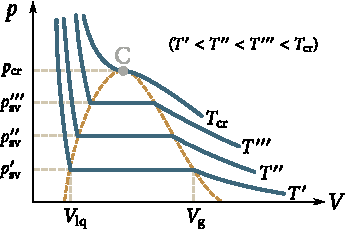
\includegraphics[scale=1]{figures/ch_15/fig_15_4.pdf}
			\caption[]{}
			\label{fig:15_4}
		\end{center}
	\end{minipage}
	\hspace{-0.05cm}
	\begin{minipage}[t]{0.5\linewidth}
		\begin{center}
			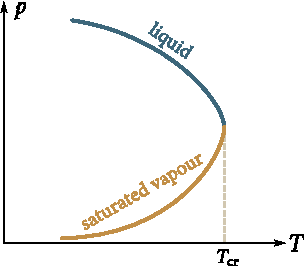
\includegraphics[scale=1]{figures/ch_15/fig_15_5.pdf}
			\caption[]{}
			\label{fig:15_5}
		\end{center}
	\end{minipage}
	\vspace{-0.4cm}
\end{figure}

%Point C is the limit which the horizontal portions of the isotherms tend to when the temperature tends to its critical value $\ab{T}{cr}$. It is called the \textbf{critical point}. The state depicted by point C is defined as the \textbf{critical state} of a substance. The volume $\ab{V}{cr}$, pressure $\ab{p}{cr}$, and temperature $\ab{T}{cr}$ corresponding to the critical state are called \textbf{critical quantities}. Point C is a point of inflection for the critical isotherm. A tangent to the isotherm at point C is parallel to the $V$-axis.
Điểm $K$ là giới hạn, mà các đoạn thẳng nằm ngang của các đường đẳng nhiệt sẽ đạt tới khi nhiệt độ tiến dần tới nhiệt độ tới hạn $\ab{T}{th}$, được gọi là \textbf{điểm tới hạn}. Trạng thái được biểu diễn bằng điểm $K$ được gọi là \textbf{trạng thái tới hạn} của chất. Thể tích $\ab{V}{th}$, áp suất $\ab{p}{th}$ và nhiệt độ $\ab{T}{th}$ được gọi là các \textbf{đại lượng tới hạn}. Đối với đường đẳng nhiệt tới hạn thì điểm $K$ là điểm uốn. Đường tiếp tuyến với đường đẳng nhiệt ở điểm $K$ nằm song song với trục $V$.\\

%It can be seen from \fig{15_4} that the saturated vapour pressure grows with the temperature and reaches the value $\ab{p}{cr}$ at the critical temperature. At temperatures above the critical one, the concept of a saturated vapour loses its meaning. Therefore, the curve showing the temperature dependence of the saturated vapour pressure terminates at the critical point (see \fig{15_2}).
Từ \fig{15_4} suy ra áp suất hơi bão hòa tăng theo nhiệt độ. Ở nhiệt độ tới hạn nó đạt tới giá trị $\ab{p}{th}$. Ở nhiệt độ cao hơn nhiệt độ tới hạn thì khái niệm bão hòa mất hết ý nghĩa. Vì vật đường cong biểu diễn sự phụ thuộc của áp suất hơi bão hòa vào nhiệt độ chấm dứt ở điểm tới hạn (xem \fig{15_2}).\\

%If we draw a line through the extreme points of the horizontal portions of the isotherms (\fig{15_4}), we get a bell-shaped curve confining the region of two-phase states of a substance. At above critical temperatures, a substance is homogeneous at any pressure. At such temperatures, a substance cannot be liquefied, no matter what pressure is applied to it.
Nếu ta vẽ một đường đi qua những điểm nút của các đoạn nằm ngang của các đường đẳng nhiệt (\fig{15_4}) thì ta được một đường cong hình chuông; đường cong này giới hạn vùng các trạng thái hai pha của chất. Ở những nhiệt độ cao hơn nhiệt độ tới hạn thì, dưới bất cứ áp suất nào, chất cũng là đồng tính. Ở những nhiệt độ đó không có cách nén nào có thể làm cho chất hóa lỏng được.\\

%The concept of the critical temperature was first introduced in 1860 by the Russian scientist Dmitri Mendeleev (1834-1907). He called it the temperature of absolute boiling of a liquid and considered it as the temperature at which the forces of cohesion between the molecules vanish, and a liquid transforms into a vapour regardless of its pressure and the volume it occupies.
Khái niệm nhiệt độ tới hạn lần đầu tiên được D.I.Mendeleev (1834-1907) đưa ra vào năm 1860. Mendeleev gọi nhiệt độ đó là nhiệt độ sôi tuyệt đối của chất lỏng và xét nó như nhiệt độ tại đó biến mất lực liên kết giữa các phân tử và chất lỏng được biến thành hơi không phụ thuộc gì vào áp suất và thể tích mà nó chiếm.\\

\begin{figure}[!htb]
	\begin{minipage}[t]{0.5\linewidth}
		\begin{center}
			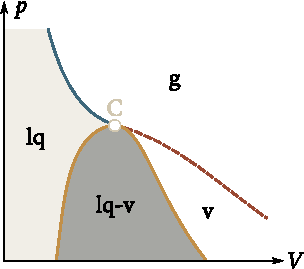
\includegraphics[scale=1]{figures/ch_15/fig_15_6.pdf}
			\caption[]{}
			\label{fig:15_6}
		\end{center}
	\end{minipage}
	\hspace{-0.05cm}
	\begin{minipage}[t]{0.5\linewidth}
		\begin{center}
			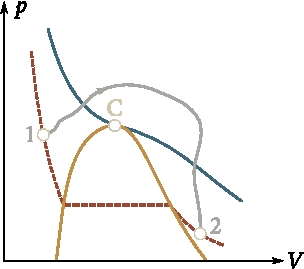
\includegraphics[scale=1]{figures/ch_15/fig_15_7.pdf}
			\caption[]{}
			\label{fig:15_7}
		\end{center}
	\end{minipage}
	\vspace{-0.4cm}
\end{figure}

%The bell-shaped curve and the portion of the critical isotherm to the left of point C divide the $p$-$V$ diagram into three regions (\fig{15_6}). The light-shaded area shows the region of homogeneous liquid states of a substance. Under the bell-shaped curve is the region of two-phase states, and, finally, the region to the right of the bell-shaped curve and the upper branch of the critical isotherm is the region of homogeneous gaseous states of a substance. In the latter region, we can earmark the part under the right-hand branch of the critical isotherm and call it the vapour region. Any state in this region differs from the other gaseous states in that upon isothermal compression the substance which was originally in this state is liquefied. The substance in one of the states at a temperature above the critical one cannot be liquefied, no matter what pressure is applied. It is not customary practice to divide the gaseous states into a gas and a vapour.
Đường cong hình chuông và đoạn của đường đẳng nhiệt tới hạn nằm bên trái điểm $K$ chia giản đồ ($p,V$) thành ba miền (\fig{15_6}). Miền có màu sáng là miền những trạng thái lỏng đồng tính của chất. Phần dưới đường cong hình chuông là miền các trạng thái hai pha, và cuối cùng, phần nằm bên phải của đường cong hình chuông và nhánh trên của đường đẳng nhiệt tới hạn là miền các trạng thái khi đồng tính của chất. Trong miền này có thể tách ra một phần đặc biệt nằm dưới nhánh phải của đường đẳng nhiệt tới hạn mà ta gọi là miền hơi. Bất kỳ trạng thái nào ở trong miền này cũng khác những trạng thái khí còn lại ở chỗ là khi ta nén đẳng nhiệt chất hơi ở trạng thái đó thì nó sẽ bị hóa lỏng. Chất khí ở một trạng thái có nhiệt dộ cao hơn nhiệt độ tới hạn đều không có cách nào có thể nén để hóa lỏng được. Việc tách các trạng thái khí ra khí và hơi chưa được toàn thể mọi người thừa nhận.\\

%Having selected a transition process so that it does not intersect a two-phase region (\fig{15_7}), we can ensure a transition from the liquid state to the gaseous one (or vice versa) without separation of the substance into two phases. In this case, the substance will remain homogeneous all the time in the course of the transition process.
Bằng cách chọn quá trình chuyển sao cho nó không cắt miền hai pha (\fig{15_7}), ta có thể thực hiện được sự chuyển từ trạng thái lỏng sang trạng thái khí (hoặc ngược lại) mà không cần quá trình tách chất ra thành hai pha. Trong trường hợp này trong quá trình chuyển chất sẽ luôn luôn là đồng tính.

\section{Hơi quá bão hòa và chất lỏng quá nóng}\label{sec:15_5}

%Section~\ref{sec:10_13} gives \eqn{10_62} proposed by van der Waals to describe the state of gases at high densities. Figure~\ref{fig:15_8} depicts van der Waals isotherms, \ie, curves described by \eqn{10_62} for several temperatures. A characteristic of these isotherms is the fact that at temperatures not exceeding the value $\ab{T}{cr}$. the curves have an S-shaped bend in whose region three different values of the volume correspond to a given pressure. Real isotherms (see \fig{15_4}) do not have such a bend, but have a straight horizontal portion instead of it. In \fig{15_9}, a real isotherm and a van der Waals isotherm are superposed on one another. The van der Waals equation describes the path of the isotherm quite well at volumes exceeding $\ab{V}{g}$. At volumes smaller than $\ab{V}{lq}$, the path of a real isotherm also approximately follows the van der Waals equation. Thus, this equation covers not only the gaseous, but also the liquid state of a substance.
Trong mục \ref{sec:10_13} ta đã dẫn ra \eqn{10_62} của Van der Waals mô tả trạng thái của các chất khí có những mật độ lớn. Trên hình \ref{fig:15_8} ta cẽ những đường đẳng nhiệt Van der Waals tức là những đường cong mô tả bởi \eqn{10_62} ứng với một vài nhiệt độ. Điều đặc biệt của những đường đẳng nhiệt này là ở những nhiệt độ thấp hơn giá trị $\ab{T}{th}$ trên các đường cong có đoạn uốn cong hình chữ S; trong vùng này ứng với một giá trị đã cho của áp suất có ba giá trị khác nhau của thể tích. Ở các đường đẳng nhiệt thực (xem \fig{15_4}) không có đoạn uốn cong đó; thay cho đoạn uốn cong, ở các đường đó có đoạn thẳng nằm ngang. Trên hình \fig{15_9} ta vẽ một đường đẳng nhiệt thực chồng lên một đường đẳng nhiệt Van der Waals mô tả khá tốt dạng của đường đẳng nhiệt ở những thể tích lớn hơn $\ab{V}{k}$. Ở những thể tích nhỏ hơn $\ab{V}{l}$, dạng của đường đẳng nhiệt thực cũng tuân theo gần đúng phương trình Van der Waals. Vì vậy phương trình này bao quát không những trạng thái khí mà cả trạng thái lỏng của chất.\\

\begin{figure}[t]
	\begin{minipage}[t]{0.5\linewidth}
		\begin{center}
			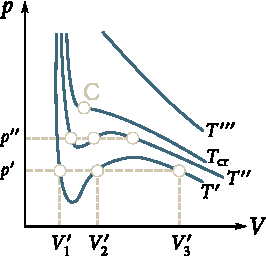
\includegraphics[scale=1]{figures/ch_15/fig_15_8.pdf}
			\caption[]{}
			\label{fig:15_8}
		\end{center}
	\end{minipage}
	\hspace{-0.05cm}
	\begin{minipage}[t]{0.5\linewidth}
		\begin{center}
			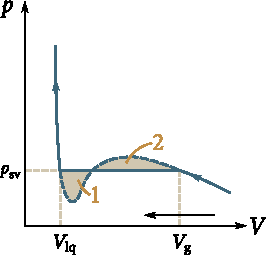
\includegraphics[scale=1]{figures/ch_15/fig_15_9.pdf}
			\caption[]{}
			\label{fig:15_9}
		\end{center}
	\end{minipage}
	\vspace{-0.4cm}
\end{figure}

%It can be seen from a comparison of a van der Waals isotherm with a real one that these isotherms approximately coincide on portions corresponding to one-phase states of a substance, but behave absolutely differently in the region of separation into two phases. Instead of the S-shaped bend on the van der Waals isotherm, the real isotherm has a straight horizontal portion in this region which is located so that the shaded areas 1 and 2 enclosed by the bend (\fig{15_9}) are the same.
Từ việc đối chiếu đường đẳng nhiệt Van der Waals với đường đẳng nhiệt thực, ta suy ra là các đường đẳng nhiệt đó trùng nhau ở những đoạn ứng với những trạng thái một pha của chất, nhưng chúng hoàn toàn khác nhau ở miền mà chất bị tách thành hai pha. Thay cho đoạn uốn cong hình chữ S trên dường đẳng nhiệt Van der Waals, đường đẳng nhiệt thực có đoạn thẳng nằm ngang mà ở miền đó, đoạn này nằm sao cho diện hình được tô đậm 1 và 2 nằm giữa đoạn đó và các đoạn uốn khúc là như nhau (\fig{15_9}).\\

%Separation into two phases is explained by the lack of stability of the homogeneous states corresponding to bend $1$-$2$-$3$-$4$ (\fig{15_10}). The instability of the states between points $2$ and $3$ becomes obvious if we take into account that the derivative $\diffin{p}{V}$ is positive on this part of the bend. Hence, a substance capable of passing consecutively through states $2$-$3$ would have absolutely unnatural properties: an increase in the volume of the gas would be attended by a growth in pressure instead of a reduction in it.
Sự tách thành hai pha được giải thích bằng sự không ổn định của những trạng thái đồng tính ứng với đoạn đường cong $1-2-3-4$ (\fig{15_10}). Tính không ổn định của các trạng thái trên đoạn $2-3$ là rất hiển nhiên, vì trên đoạn đó đạo hàm $\diffin{p}{V}$ là dương. Do đó chất có khả năng đi theo chuỗi những trạng thái $2-3$ hình như có những tính chất hoàn toàn phi lý: sự tăng thể tích của chất khí lại kèm theo sự tăng áp suất chứ không phải là giảm.\\


\begin{figure}[!htb]
	\begin{center}
		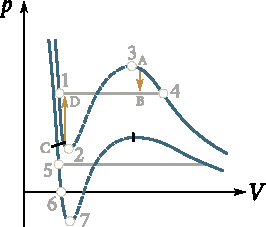
\includegraphics[scale=1]{figures/ch_15/fig_15_10.pdf}
		\caption[]{}
		\label{fig:15_10}
	\end{center}
	\vspace{-0.8cm}
\end{figure}

%The derivative $\diffin{p}{V}$ is negative on parts $1$-$2$ and $3$-$4$, so that it would seem possible for these portions of the curve to be realized. Indeed, in certain conditions, the states corresponding to these portions can be achieved. True, they are not fully stable: for example, it is sufficient for a dust particle to get into the vapour in state A for the substance to break up into two phases and pass over into state B (see the transition A $\to$ B shown by the arrow in \fig{15_10}). Such not fully stable states are called \textbf{metastable}. The substance in states $1$-$2$ is called a \textbf{superheated liquid}, and in states $3$-$4$ is called a \textbf{supersaturated vapour}.
Trên đoạn $1-2$ và $3-4$ thì $\diffin{p}{V}$ âm, nên hình như những đoạn đó có thể là hiện thực. Thực vậy, trong những điều kiện đặc biệt ta có thể thực hiện được những trạng thái ứng với những đoạn đó. Đúng là những trạng thái đó không phải là ổn định: chỉ cần, chẳng hạn, ở trạng thái $A$ cho rơi vào hơi những hạt bụi nhỏ là toàn bộ chất đó bị tách thành hai pha và chuyển sang trạng thái $B$ (xem sự chuyển $A \to B$ chỉ bằng mũi tên trên \fig{15_10}). Những trạng thái hoàn toàn không bền vững như vậy gọi là những \textbf{trạng thái siêu bền}. Chất ở những trạng thái $1-2$ gọi là những \textbf{Chất lỏng quá nóng}; chất ở những trạng thái $3-4$ gọi là \textbf{hơi quá bão hòa}.\\

%At sufficiently low temperatures, the bottom part of the bend in the van der Waals isotherm crosses the $V$-axis and passes into the region of negative pressures (see the bottom isotherm in \fig{15_10}). A substance under a negative pressure is obviously in a state of tension instead of compression. Such states can also be realized in certain conditions. Thus, portion $5$-$6$ on the bottom isotherm corresponds to a \textbf{superheated liquid}, and $6$-$7$ to a \textbf{tensioned liquid}.
Ở những nhiệt độ khá thấp phần dưới của đoạn uốn khúc của đường đẳng nhiệt Van der Waals sẽ cắt trục $V$ và đi vào miền những áp suất âm (xem đường đẳng nhiệt nằm dưới ở \fig{15_10}). Chất dưới áp suất âm, dĩ nhiên, ở trạng thái không bị nén và dãn. Trong những điều kiện đặc biệt, ta cũng có thể thực hiện được những trạng thái như vậy. Vì vậy, đoạn $5-6$ trên đường đẳng nhiệt nằm dưới ứng với \textbf{chất lỏng quá nóng}, còn đoạn $6-7$ ứng với \textbf{chất lỏng bị dãn}.\\

%Let us consider the conditions in which metastable states can be brought about. We shall begin with a supersaturated vapour. If a vapour contains absolutely no foreign inclusions, its condensation into a liquid cannot begin. For a droplet to form, a great number of molecules must simultaneously approach one another to a distance of the same order as the distances between the molecules in the liquid, and this is absolutely improbable. For condensation to commence, the presence of so-called \textbf{condensation centres} is needed, which capture the molecules flying toward them and transfer them into the condensed phase. Dust particles, liquid droplets, and, especially, charged particles (ions) can be condensation centres.
Ta xét những điều kiện trong đó có thể thực hiện được những trạng thái siêu bền. Ta bắt đầu bằng hơi quá bão hòa. Nếu hơi hoàn toàn không chứa những hợp phần ngoại lai thì nó không thể bắt đầu ngưng tụ thành chất lỏng được. Để hình thàng những giọt nhỏ thì cần một lượng lớn các phân tử đồng thời gần nhau một khoảng vào cớ khoảng cách giữa các phân tử trong chất lỏng mà điều đó hoàn toàn không có khả năng. Để cho sự ngưng tụ có thể xảy ra, cần phải có những \textbf{tâm ngưng tụ}, những tâm này thu hút những phân tử bay về phía nó và chuyển chúng sang trạng thái ngưng tụ. Tâm ngưng tụ có thể là những hạt bụi, những giọt nhỏ chất lỏng và, đặc biệt, là những hạt điện tích (những ion).\\

%Thus, if a vapour is thoroughly purified of foreign inclusions and ions, it can be at a pressure exceeding the saturated vapour pressure $\ab{p}{sv}$ at the given temperature. This state will be metastable: it is sufficient for even one condensation centre to appear, and the state of a supersaturated vapour will be violated---the substance will pass over into a two-phase state.
Vì vậy, nếu ta làm sạch cẩn thận chất hơi khỏi những thành phần ngoại lai và những ion thì hơi đó có thể tồn tại dưới áp suất lớn hơn áp suất hơi bão hòa $\ab{p}{bh}$ ở nhiệt độ đã cho. Trạng thái đó sẽ là trạng thái siêu bền: chỉ cần xuất hiện một tâm ngưng tụ là trạng thái hơi quá bão hòa lập tức bị phá huỷ và chất chuyển sang trạng thái hai pha.

%In practice, a supersaturated vapour can be obtained by subjecting one that is not supersaturated to sharp expansion. The rapid expansion occurs without heat exchange with the surroundings and is attended by cooling of the vapour. The point depicting the state of the vapour moves along an adiabat. The latter, as was shown in \sect{10_10}, is steeper than an isotherm. Hence, the vapour can pass over from stable state $1$ corresponding to the temperature $T_1$ (\fig{15_11}) to metastable state $2$ corresponding to the lower temperature $T_2$. Such a process is used in a Wilson cloud chamber---a device intended for observing the traces of charged particles (for example, alpha particles). The air saturated with water or alcohol vapour contained in a Wilson chamber is sharply expanded. The result is cooling of the air, and the vapour becomes supersaturated. A particle flying into the chamber ionizes the molecules along its path. The supersaturated vapour condenses on the ions produced in minute droplets and forms a well visible trace.
Thực tế ta có thể thu được hơi quá bão hòa bằng cách làm dãn nở đột ngột hơi chưa quá bão hòa. Sự dãn nở nhanh diễn ra không có sự trao đổi nhiệt với môi trường chung quanh sẽ kèm theo sự làm lạnh chất hơi. Khi đó điểm biểu diễn trạng thái hơi dịch chuyển theo một đường đoạn nhiệt. Như đã nói rõ ở \sect{10_10}, đường đoạn nhiệt dốc hơn đường đẳng nhiệt; kết quả là hơi có thể chuyển từ trạng thái bền vững $1$ ứng với nhiệt độ $T_1$ (\fig{15_11}) sang trạng thái siêu bền $2$ ứng với nhiệt độ thấp hơn $T_2$. Quá trình đó được sử dụng trong buồng Wilson; đó là dụng cụ dùng để qua sát vết của các hạt điện tích (ví dụ: hạt $\alpha$). Không khí, hơi nước bão hòa hoặc rượu chứa trong buồng Wilson bị làm dãn nở đột ngột. Kết quá là không khí bị lạnh đi và hơi chuyển sang trạng thái quá bão hòa. Một hạt bay vào buồng sẽ gây ra sự ion hóa các phân tử trên đường đi của nó. Tại những ion sinh ra, hơi quá bão hòa bị ngưng tụ thành những giọt nhỏ, tạo thành một vết trong thấy được.\\

%Let us consider the conditions for obtaining a superheated liquid. The process of violent vaporization (\ie, boiling) can occur, like the process of condensation, on foreign inclusions, for example, on sand particles or gas bubbles dissolved in the liquid. If a liquid is thoroughly purified of solid inclusions and dissolved gases, then by heating it can be brought into a state with a pressure below $\ab{p}{sv}$ at a given temperature without the liquid boiling. This will be the state of a superheated liquid.
Ta hãy xét điều kiện để thu được chất lỏng quá nóng. Cũng như quá trình ngưng tụ, quá trình tạo thành hơi một cách mãnh liệt (tức là sự sôi) chỉ có thể xảy ra tại những hợp phần ngoại lai, chẳng hạn tại những hạt bụi nhỏ hay những bọt khí hòa tan trong chất lỏng. Nếu chất lỏng được làm sạch cẩn thận khỏi những thành phần rắn ngoại lai và những chất khí hòa tan trong đó thì khi nung nóng nó ta có thể đưa nó đến trạng thái có áp suất nhỏ hơn áp suất $\ab{p}{bh}$ ở nhiệt độ đã cho mà chất lỏng vẫn không sôi. Đó là trạng thái của chất lỏng quá nóng.\\

%The transition of a liquid from its conventional state to a superheated one is shown in \fig{15_12} (see transition $1$-$2$ shown by the arrow). The state of a superheated liquid is metastable. It is sufficient to throw a sand particle into a superheated liquid for the latter to boil and the substance to pass over into the stable two-phase state (see transition $C$-$D$ in \fig{15_10}).
Sự chuyển của chất lỏng từ trạng thái bình thường sang trạng thái quá nóng được vẽ trên \fig{15_12} (xem sự chuyển $1-2$ được chỉ bằng một mũi tên). Trạng thái quá nóng của chất lỏng là trạng thái siêu bền. Chỉ cần ném vào trong chất lỏng quá nóng một hạt bụi cũng đủ làm cho chất lỏng bắt đầu sôi và chueyern sang trạng thái hai pha bền vững (xem sự chuyển $C-D$ trên \fig{15_10}).

\begin{figure}[!htb]
	\begin{minipage}[t]{0.5\linewidth}
		\begin{center}
			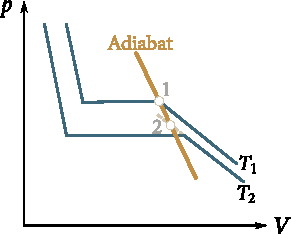
\includegraphics[scale=1]{figures/ch_15/fig_15_11.pdf}
			\caption[]{}
			\label{fig:15_11}
		\end{center}
	\end{minipage}
	\hspace{-0.05cm}
	\begin{minipage}[t]{0.5\linewidth}
		\begin{center}
			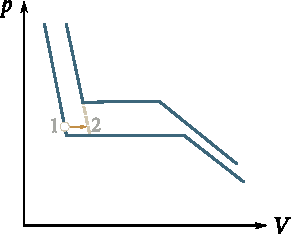
\includegraphics[scale=1]{figures/ch_15/fig_15_12.pdf}
			\caption[]{}
			\label{fig:15_12}
		\end{center}
	\end{minipage}
	\vspace{-0.4cm}
\end{figure}

%A tensioned liquid, for example, mercury, can be obtained as follows. If we submerge a long glass tube soldered at one end into mercury and, after turning it with its soldered end upward, carefully pull it out from the mercury, then we can get a column of mercury in the tube that considerably exceeds \SI{760}{\milli\metre}. Hence, the mercury will be kept in the tube not by the force of atmospheric pressure, but by the cohesion between its molecules. The mercury in the tube will be in a state of tension, \ie, under a negative pressure.
Ta có thể thu được chất lỏng bị kéo dãn, chẳng hạn thủy ngân, bằng cách sau, Nếu ta nhúng vào thủy ngân một ống thủy tinh dài hàn kín một đầu, rồi quay lại hàn kín lên phía trên và cẩn thận đưa ống đó ra ngoài thì trong ống đó có thể có một cột thủy ngân dài hơn \SI{760}{\milli\metre} rất nhiều. Do đó, thủy ngân ở trong ống sẽ chịu tác dụng không phải áp lực của khí quyển mà là lực liên kết giữa các phân tử của nó. Thủy ngân trong ống sẽ ở trạng thái bị kéo dãn, tức là dưới áp suất âm.\\

\section{Sự nóng chảy và sự kết tinh}\label{sec:15_6}

%The transition of a crystalline body to the liquid state takes place at a definite temperature for every substance and requires the expenditure of a certain amount of heat called the \textbf{heat of fusion}.
Sự chuyển của một vật chất kết tinh sang trạng thái lỏng diễn ra ở một nhiệt độ nhất định đối với mỗi một chất và tiêu thụ một nhiệt lượng nhất định gọi là \textbf{nhiệt nóng chảy}.\\

%If a substance originally in the crystalline state receives the same amount of heat every second, its temperature will change with time as shown in \fig{15_13}. First the temperature of the body will constantly grow. When the melting point $\ab{T}{m}$ is reached (point $1$ in \fig{15_13}), the temperature of the body will stop changing although the supply of heat to it is continued. At the same time, the process of melting of the solid body begins, during which new and new portions of the substance transform into a liquid. After the melting process is completed and all of the substance melts (point $2$ in \fig{15_13}), the temperature again begins to rise.
Nếu mỗi giây ta cung cấp cho một vật ban đầu ở trạng thái kết tinh một nhiệt lượng nhất định thì sự biến thiên nhiệt độ của vật theo thời gian sẽ giống như điều ta vẽ trên \fig{15_13}. Thoạt tiên, nhiệt độ của vật tăng theo thời gian. Khi đạt đến nhiệt độ nóng chảy $\ab{T}{nc}$ (điểm $1$ trên \fig{15_13}) thì mặc dầu ta vẫn tiếp tục cung cấp nhiệt cho vật như trước, nhiệt độ của vật không thay đổi nữa. Đồng thời quá trình nóng chảy của vật rắn bắt đầu, trong quá trình này các phần của vật rắn dần dần biến thành chất lỏng. Sau khi quá trình nóng chảy chấm dứt toàn thể vật hoàn toàn chuyển sang trạng thái lỏng (điểm $2$ trên \fig{15_13}) nhiệt độ lại bắt đầu tăng lên.\\

%The heating curve of an amorphous body is different (see the dash curve in \fig{15_13}). Upon the uniform supply of heat, the temperature of an amorphous body continuously grows. Amorphous bodies have no definite temperature of transition to the liquid state. This transition occurs continuously, and not in a jump. We can only indicate the temperature interval within which a body softens. The explanation is that liquids and amorphous bodies differ only in the degree of mobility of their molecules---amorphous bodies, as already indicated, are greatly supercooled liquids.
Đường cong nung nóng của vật vô định hình trông khác hẳn (xem đường cong chấm chấm trên \fig{15_13}). Khi được cung cấp nhiệt một cách đều đặn, nhiệt độ của vật vô định hình tăng lên liên tục. Đối với các vật vô định hình, không có nhiệt độ xác định của sự chuyển sang trạng thái lỏng. Sự chuyển đó được thực hiện một cách liên tục, không phải bằng một bước nhảy. Ta chỉ có thể nói về khoảng nhiệt độ trong đó vật bị chảy nhão ra. Điều đó được giải thích là giữa chất lỏng và vật vô định hình chỉ khác nhau ở độ linh động của các phân tử --- như ta đã nhận xét, những vật vô định hình là những chất lỏng bị đông lạnh rất mạnh.\\

%The melting point depends on the pressure. Thus, the transition from a crystalline to a liquid state occurs in quite definite conditions characterized by the values of the pressure and temperature. A curve in a $p$-$T$ diagram called the melting or fusion curve corresponds to a combination of these values. The melting curve is very steep. To change the melting point of ice by one kelvin, for example, the pressure has to be changed by \SI{132}{\atm}.
Nhiệt độ nóng chảy phụ thuộc vào áp suất. Vì vậy, sự chuyển từ trạng thái kết tinh sang trạng thái lỏng diễn ra trong những điều kiện hoàn toàn xác định đặc trưng bằng những giá trị của áp suất và nhiệt độ. Tập hợp những giá trị đó tạo thành một đường cong trong giản đồ ($p,T$) gọi là \textbf{đường nóng chảy}. Đường nóng chảy đi rất dốc. Chẳng hạn để làm thay đổi nhiệt độ nóng chảy của nước đá đi $1$K thì cần phải thay đổi áp suất đi \SI{132}{\atm}.\\ 

%A point on the melting curve determines the conditions in which the crystalline and the liquid phases can be in equilibrium with each other. Such equilibrium is possible with any ratio between the masses of the liquid and the crystals, \ie, at values of the volume of the system within the limits from $m\ab{V}{s}'$ to $m\ab{V}{lq}'$, where $m$ is the mass of the system, and $\ab{V}{s}'$ and $\ab{V}{lq}'$ are the specific volumes of the solid and the liquid phases. Consequently, in a $p$-$V$ diagram, a portion of a horizontal straight line (\fig{15_14}) corresponds to every point of a melting curve. Since the substance in the states depicted by points on this line has the same temperature, straight line $1$-$2$ in \fig{15_14} is a portion of an isotherm corresponding to two-phase states of the substance (compare with the horizontal portions of the isotherms in \fig{15_14}).
Những điểm của đường nóng chảy xác định những điều kiện trong đó pha kết tinh và pha lỏng có thể đứng cân bằng với nhau. Sự cân bằng đó có thể xảy ra ở mọi tỷ lệ giữa khối lượng chất lỏng và khối lượng tinh thể, tức là với các giá trị của thể tích của hệ nằm trong khoảng giới hạn từ $m\ab{V}{r}'$ đến $m\ab{V}{l}'$, trong đó $m$ là khối lượng của hệ còn $\ab{V}{r}'$ và $\ab{V}{l}'$ là những thể tích riêng của pha rắn và pha lỏng. Vì vậy mỗi một điểm trên đường nóng chảy ứng với một đoạn thẳng nằm ngang trên giản đồ ($p,V$) (\fig{15_14}). Vì rằng chất ở trong các trạng thái biểu diễn bằng những điểm trên đoạn thẳng đó có cùng một nhiệt độ, nên đường thẳng $1-2$ trên \fig{15_14} chính là một đoạn của đường đẳng nhiệt ứng với những trạng thái hai pha của chất ( so sánh với những đoạn nằm ngang của các đường đẳng nhiệt trên \fig{15_14}).\\

\begin{figure}[!htb]
	\begin{minipage}[t]{0.5\linewidth}
		\begin{center}
			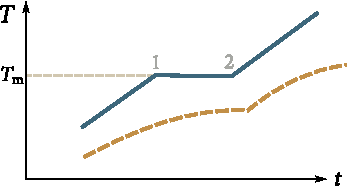
\includegraphics[scale=1]{figures/ch_15/fig_15_13.pdf}
			\caption[]{}
			\label{fig:15_13}
		\end{center}
	\end{minipage}
	\hspace{-0.05cm}
	\begin{minipage}[t]{0.5\linewidth}
		\begin{center}
			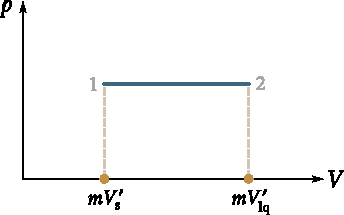
\includegraphics[scale=1]{figures/ch_15/fig_15_14.pdf}
			\caption[]{}
			\label{fig:15_14}
		\end{center}
	\end{minipage}
\end{figure}

%The process of crystallization that is the reverse of melting proceeds as follows. When a liquid is cooled to a temperature at which the solid and liquid phases can be in equilibrium at the given pressure (\ie, to the same temperature at which melting occurs), the simultaneous growth of minute crystals begins about the so-called \textbf{nuclei} or \textbf{centres of crystallization}. Growing larger and larger, the separate crystals in the long run join one another, forming a polycrystalline solid.
Quá trình kết tinh, ngược với quá trình nóng chảy, xảy ra như sau. Khi làm lạnh chất lỏng đến nhiệt độ tại đó pha rắn và pha lỏng có thể đứng cân bằng với nhau ở áp suất đã cho (tức là chính nhiệt độ tại đó xảy ra sự nóng chảy) thì sự mọc ra cùng một lúc những tinh thể nhỏ tinh thể nhỏ xung quanh những \textbf{mầm} hoặc là những \textbf{tâm kết tinh}. Được bắt đầu từ những tinh thể nhỏ riêng biệt mọc càng ngày càng nhiều và cuối cùng chúng nối liền lại với nhau để tạo thành một vật rắn đa tinh thể.\\

%Solid particles suspended in the liquid can be the crystallization centres. A liquid thoroughly purified of such particles can be cooled to below the freezing point without the formation of crystals beginning. The state of such a supercooled liquid is metastable. It is usually sufficient for a dust particle to get into such a liquid for it to break up into a liquid and crystals at the equilibrium temperature. Sometimes upon great supercooling, however, the mobility of the liquid molecules is so insignificant that the metastable state can be preserved for a very long time. The liquid in such cases has a very low fluidity and is an amorphous solid. 
Tâm kết tinh có thể là những hạt rắn lơ lửng trong chất lỏng. Nếu chất lỏng được làm sạch cẩn thận cho hết những hạt như vậy thì ta có thể làm lạnh cho nó tới nhiệt độ thấp hơn nhiệt độ kết tinh mà vẫn chưa bắt đầu tạo thành những tinh thể nhỏ. Trạng thái lạnh như vậy của chất lỏng là trạng thái siêu bền. Thông thường chỉ cần một hạt bụi nhỏ rơi vào chất lỏng đó là lập tức nó bị phân ra thành chất lỏng và các tinh thể nằm ở nhiệt độ cân bằng. Tuy nhiên, trong một số trường hợp, khi làm lạnh rất mạnh, độ linh động của các phân tử có thể giữ được rất lâu. Trong những trường hợp đó, chất lỏng có độ lưu rất nhỏ và nó chính là một vật rắn vô định hình.\\

%The process of crystallization is attended by the liberation of the same amount of heat as that absorbed in melting.
Quá trình kết tinh kèm theo sự tỏa ra một nhiệt lượng đúng bằng nhiệt lượng hấp thụ khi nóng chảy.


\section{Phương trình Clapeyron - Clausius}\label{sec:15_7}

%We saw in the preceding sections that any two phases of a substance can be in equilibrium only at a definite pressure whose magnitude depends on the temperature. We can obtain the general form of this relation by resorting to the concept of entropy. For this purpose, we shall consider a Carnot cycle for a system consisting of two phases of a given substance in equilibrium.
Trong những mục trước chúng ta đã thấy rõ là hai pha chất bất kỳ của một chất chỉ có thể nằm cân bằng với nhau ở một áp suất nhất định, độ lớn của áp suất phụ thuộc vào nhiệt độ. Ta có thể thu được dạng tổng quát của sự phụ thuộc đó nếu dùng khái niệm entropy. Muốn vậy ta hãy xét chu trình Carnot của hệ gồm hai pha của chất đã cho nằm cân bằng với nhau.\\

%In a $p$-$V$ diagram, the Carnot cycle for a two-phase system has the form shown in \fig{15_15} (the temperatures of the high temperature and low temperature reservoirs are assumed to differ by the very small value $\Delta T$). The numbers $1$ and $2$ denote the extreme points of the horizontal portion of the isotherm of temperature $T$. States $1$ and $2$ are one-phase ones. All the intermediate points on $1$-$2$, depict two-phase states differing from each other in the distribution of the mass of the substance between the first and the second phases.
Trên giản đồ ($p,V$) chu trình Carnot của hệ hai pha có dạng vẽ trên \fig{15_15} (nhiệt độ của nguồn nóng và nguồn lạnh giả thử khác nhau một rất nhỏ $\Delta T$). Các số $1$ và $2$ chỉ những điểm đầu mút của đoạn nằm ngang của đường đẳng nhiệt ở nhiệt độ $T$. Các trạng thái $1$ và $2$ là các trạng thái một pha. Tất cả những điểm trung gian của đoạn thẳng $1-2$ biểu diễn những trạng thái hai pha; những trạng thái này khác nhau về sự phân bố khố lượng của chất giữa pha thứ nhất và pha thứ hai.\\

\begin{figure}[!htb]
	\begin{center}
		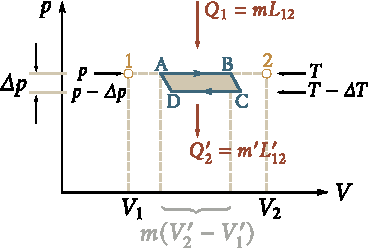
\includegraphics[scale=1]{figures/ch_15/fig_15_15.pdf}
		\caption[]{}
		\label{fig:15_15}
	\end{center}
\end{figure}

%The isothermal process A $\to$ B is attended by a phase transition of a certain mass $m$ of the substance. The volume of the substance receives an increment of $m(V_2'-V_1')$, where $V_1'$ and $V_2'$ are the specific volumes of the first and second phases. For such a transition to occur, the heat $Q_1$ equal to $mL_{12}$ must be supplied to the substance ($L_{12}$ is the specific heat absorbed in the transition from state $1$ to state $2$ at the temperature $T$). The heat $Q_1$ is the heat which the system receives in the course of the cycle from the high temperature reservoir. The heat is given up to the low temperature reservoir in the course of the isothermal process C $\to$ D. The heat given up amounts to $Q_2'=m'L_{12}'$, where $L_{12}'$ is the heat of transition $1$-$2$ at the temperature $T-\Delta T$, and $m'$ is the mass of the substance experiencing a phase transition in the course of the process C $\to$ D. This value differs somewhat from $m$ because a certain mass of the substance undergoes phase transitions in the course of adiabatic processes.
Quá trình đẳng nhiệt $A \to B$ đi đôi với sự biến đổi pha của một khối lượng $m$ nào đó của chất. Khi đó thể tích của chất có một số gia bằng $m(V_2'-V_1')$, trong đó $V_1'$ và $V_2'$ là những thể tích riêng của pha thứ nhất và pha thứ hai. Muốn cho sự biến đổi pha đó có thể thực hiện được thì cần phải cung cấp cho chất đó một nhiệt lượng là $Q_1$ bằng $mq_{12}$, trong đó $q_{12}$ là ẩn nhiệt bị hấp thụ trong sự chuyển từ trạng thái $1$ sang trạng thái $2$ ở nhiệt độ $T$. Nhiệt lượng $Q_1$ là nhiệt lượng mà hệ thu được từ nguồn nóng của một chu trình. Trong quá trình đẳng nhiệt $C \to D$ thì nhiệt lượng tỏa cho nguồn lạnh. Nhiệt lượng tỏa ra bằng $Q_2'=m'q_{12}'$, trong đó $q_{12}'$ là ẩn nhiệt của sự chuyển $1-2$ ở nhiệt độ $T-\Delta T$, còn $m'$ là khối lượng của chất chịu sự biến đổi pha trong quá trình $C \to D$. Đại lượng này khác khối lượng $m$ một chút, vì rằng đã có một khối lượng nào đó của chất này chịu những sự biến đổi pha trong những quá trình đoạn nhiệt.\\

%On ihe isothermal portion A-B, the entropy of the system receives the increment $\Delta S_1$ equal to $Q_1/T$. On the isothermal portion C-D, the increment of the entropy is $\Delta S_2=-Q_2'(T-\Delta T)$. The entropy does not change in the course of the adiabatic processes B-C and D-A. The total increment of the entropy during a cycle is zero. Hence,
Trên đoạn đẳng nhiệt $A-B$, entropy của hệ thu được một số gia $\Delta S_1$  bằng $Q_1/T$. Trên đoạn đẳng nhiệt $C-D$, số gia của entropy bằng $\Delta S_2=-Q_2'(T-\Delta T)$. Trong những quá trình đoạn nhiệt $B-C$ và $D-A$ entropy không bị thay đổi. Số gia toàn phần của entropy trong một chu trình bằng không. Do đó:

\begin{equation*}
    \Delta S_1 + \Delta S_2 = \frac{Q_1}{T} - \parenthesis{\frac{Q_2'}{T-\Delta T}} = 0
\end{equation*}

\noindent

%whence
Từ đó suy ra
\begin{equation}\label{eq:15_4}
    \parenthesis{Q_1 - Q_2'}T = Q_1 \Delta T.
\end{equation}

%According to \eqn{12_3}, $Q_1-Q_2'$ equals the work done during a cycle. This work can be found by calculating the area of the cycle. Approximately, this area can be considered equal to $m(V_2'-V_1')\Delta p$ (see \fig{15_15}). We thus arrive at the relation
Theo \eqn{12.3}, $Q_1-Q_2'$ bằng công thực hiện trong một chu trình. Ta có thể tìm được công đó bằng cách tính diện tích của chu trình. Một cách gần đúng, diện tích của chu trình có thể coi như bằng $m(V_2'-V_1')\Delta p$ (xem \fig{15_15}). Vì vậy, ta đi tới hệ thức

\begin{equation}\label{eq:15_5}
    Q_1 - Q_2' = m\parenthesis{(V_2'-V_1')}\Delta p.
\end{equation}

\noindent
%In the limit when $\Delta p$ tends to zero (for which it is necessary that $\Delta T$ also tend to zero), expression~\eqref{eq:15_5} transforms into a strict equality.
Tại giới hạn khi $\Delta p$ tiến dần đến không (muốn vậy chỉ cần $\Delta T$ tiến đến không) thì hệ thức \eqref{eq:15_5} sẽ trở thành một đẳng thức thực sự.\\

%Let us substitute expression~\eqref{eq:15_5} in \eqn{15_4} for $Q_1-Q_2'$, and also $mL_{12}$ for $Q_1$. As a result, we get
Thay $Q_1-Q_2'$ trong \eqn{15_4}  bằng biểu thức \eqref{eq:15_5}. Ngoài ra, còn thay $Q_1$ bằng $mq_{12}$. Kết quả là ta thu được
\begin{equation*}
    m\parenthesis{V_2'-V_1'} T \Delta p \approx mq_{12} \Delta T.
\end{equation*}

\noindent
%Hence,
Từ đây suy ra

\begin{equation*}
    \frac{\Delta p}{\Delta T} \approx \frac{q_{12}}{T\parenthesis{V_2'-V_1'}}.
\end{equation*}

\noindent
%Finally, performing the limit transition $\Delta T\to 0$, we arrive at the strict equation
Cuối cùng, thực hiện việc chuyển đến giới hạn $\Delta T\to 0$, ta đi đến một đẳng thức thực sự

\begin{equation}\label{eq:15_6}
    \diff{p}{T} = \frac{q_{12}}{T\parenthesis{V_2'-V_1'}}.
\end{equation}

\noindent
%This expression is called the \textbf{Clapeyron-Clausius} equation. It relates the temperature derivative of the equilibrium pressure to the heat of transition, the temperature, and the difference between the specific volumes of the phases in equilibrium.
Hệ thức thu được gọi là \textbf{phương trình Clapeyron-Clausius}. Nó liên hệ đạo hàm của áp suất cân bằng theo nhiệt độ với nhiệt của sự chuyển với nhiệt độ và với hiệu các thể tích riêng của các pha ở trạng thái cân bằng.\\

%According to \eqn{15_6}, the sign of the derivative $\diffin{p}{T}$ depends on what change in the volume---an increase or a reduction---attends a phase transition occurring with the absorption of heat. In the evaporation of a liquid or a solid, the volume always grows, therefore $\diffin{p}{T}$ for a vaporization curve, and also for a sublimation one, can only be positive: elevation of the temperature leads to an increase in the equilibrium pressure.
Theo \eqn{15_6} dấu của đạo hàm $\diffin{p}{T}$ phụ thuộc vào điều là sự biến đổi pha mà trong đó có sự hấp thụ nhiệt được kèm theo sự biến đổi nào của thể tích nghĩa là sự tăng hay sự giảm thể tích. Khi chất lỏng hoặc chất rắn bay hơi thì thể tích bao giờ cũng tăng, vì vậy $\diffin{p}{T}$ của đường cong bay hơi cũng như của đường cong thăng hoa chỉ có thể có trị số dương: sự tăng nhiệt độ đưa đến sự tăng áp suất cân bằng.\\

%The volume grows, as a rule, in melting, so that $\diffin{p}{T}>0$: an increase in the pressure raises the melting point. For some substances including water, however, the volume of the liquid phase is less than that of the solid phase $(V_2'-V_1')$\footnote{The volume of water is known to increase when it freezes. For this reason, ice has a smaller density than water.}. In this case, $\diffin{p}{T}<0$---an increase in the pressure is attended by lowering of the melting point. We can melt ice by applying a high pressure to it without raising its temperature above \SI{0}{\degreeCelsius}.
Khi nóng chảy thì thông thường thể tích cũng tăng nên $\diffin{p}{T}>0$: sự tăng áp suất dẫn tới sự tăng nhiệt độ nóng chảy. Tuy nhiên ở một vài chất, trong đó có cả nước, thể tích của pha lỏng nhỏ hơn thể tích pha rắn $(V_2'<V_1')$ $\footnote{Ta biết rằng khi đóng băng thì thể tích của nước tăng lên. Vì nguyên nhân đó nước đá có tỷ trọng nhỏ hơn nước.}$. Trong trường hợp này $\diffin{p}{T}<0$ nghĩa là sự tăng áp suất đi đôi với sự giảm nhiệt độ nóng. Khi ép nước đá thật mạnh ta có thể làm cho nó chảy ra mà không cần tăng nhiệt độ cao hơn \SI{0}{\degreeCelsius}.

%The temperature of transition from one crystalline modification to another will rise or lower with increasing pressure depending on which of the solid phases has a greater specific volume.
Nhiệt độ của sự chuyển từ hình thức kết tinh này sang hình thức kết tinh khác sẽ được nâng lên hoặc hạ xuống khi áp suất tùy thuộc vào điều là pha rắn nào có thể tích lớn hơn

\section{Điểm ba. Giản đồ trạng thái}\label{sec:15_8}

%Let us take a substance in the form of a liquid and its saturated vapour in equilibrium with it and withdraw heat from it without changing the volume. This process will be attended by lowering of the temperature of the substance and a corresponding reduction in the pressure. Therefore, the point depicting the state of the substance in a $p$-$T$ diagram will move downward along the vaporization curve (\fig{15_16}). This will continue until the freezing point of the substance is reached corresponding to the equilibrium pressure value. Let us denote this temperature by $\ab{T}{tr}$. The temperature and the pressure remain constant all the time the freezing process goes on. The heat removed during this process is the heat liberated in freezing (crystallization).
Ta hãy lấy một chất dưới dạng chất lỏng và hơi bão hòa đứng cân bằng với nó mà không làm thay đổi thể tích khi lấy nhiệt của nó.Quá trình này sẽ đi đôi với sự giảm nhiệt độ của vật và sự giảm tương ứng của áp suất. Vì vậy điểm biểu diễn trạng thái của chất đó trong giản đồ trạng thái ($p,V$) sẽ dịch chuyển xuống phía dưới theo đường cong bay hơi (\fig{15_16}). Hiện tượng này sẽ tiếp diễn cho đến khi đạt tới nhiệt độ kết tinh của chất tương ứng với giá trị cân bằng của áp suất. Ta hãy ký hiệu nhiệt độ đó là $\ab{T}{b}$. Trong suốt thời gian diễn ra sự kết tinh, nhiệt độ và áp suất vẫn không đổi. Lúc đó nhiệt lượng bị lấy đi chính là nhiệt lượng tỏa ra khi kết tinh.\\

\begin{figure}[!htb]
	\begin{center}
		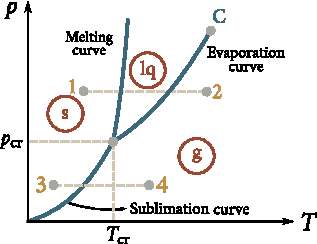
\includegraphics[scale=1]{figures/ch_15/fig_15_16.pdf}
		\caption[]{}
		\label{fig:15_16}
	\end{center}
\end{figure}

%The temperature $\ab{T}{tr}$ and the equilibrium pressure $\ab{p}{tr}$ corresponding to it are the only values of the temperature and pressure at which three phases of a substance ---the solid, liquid, and gaseous ones---can be in equilibrium. The corresponding point in a $p$-$T$ diagram is called a \textbf{triple point}. Thus, a triple point determines the conditions in which three phases of a substance can be in equilibrium simultaneously.
Nhiệt độ $\ab{T}{b}$ và áp suất $\ab{p}{b}$ ứng với nó là giá trị duy nhất của nhiệt độ và áp suất, tại đó có thể có sự cân bằng của ba pha của chất: rắn, lỏng và khí. Điểm tương ứng trên giản đồ ($p,T$) gọi là \textbf{điểm ba}. Vì vậy, điểm ba xác định bằng những điều kiện trong đó có thể có đồng thời sự cân bằng pha của ba chất.\\

%Upon completion of the freezing process, the solid and gaseous phases will be in equilibrium. If we continue to remove heat from the substance, the temperature will again begin to lower. The pressure of the vapour in equilibrium with the crystalline phase will decrease accordingly. The point depicting the state of the substance will move downward along the sublimation curve.
Khi chấm dứt quá trình kết tinh sẽ có pha rắn và pha khí nằm cân bằng. Nếu tiếp tục lấy nhiệt của vật thì nhiệt độ lại bắt đầu hạ thấp xuống. Tương ứng, áp suất hơi nằm cân bằng với ph kết tinh cũng giảm. Điểm biểu diễn trạng thái của chất dich chuyển xuống dưới dọc theo đường cong thăng hoa.\\

%The temperature of a triple point is the temperature at which a substance melts when it is under the pressure $\ab{p}{tr}$. At other pressures, the melting point will be different. The relation between the pressure and the melting point will be depicted by the melting curve beginning at the triple point. Thus, a triple point is on the intersection of three curves determining the conditions of equilibrium of two phases: solid and liquid, liquid and gaseous, and, finally, solid and gaseous.
Nhiệt độ của điểm ba là nhiệt độ tại đó chất dưới áp suất bằng $\ab{p}{b}$ bắt đầu nóng chảy. Ở những áp suất khác, nhiệt độ nóng chảy cũng sẽ khác. Mối liên hệ giữa áp suất và nhiệt độ nóng chảy được biểu diễn bằng đường cong nóng chảy bắt đầu từ điểm ba. Vì vậy, điểm ba nằm tại giao điểm của ba đường cong xác định những điều kiênh cân bằng của hai pha: rắn và lỏng; lỏng và khí và, cuối cùng, rắn và khí.\\

%Depending on the relation between the specific volumes of the solid and liquid phases, the melting curve is directed either as shown in \fig{15_16} ($\diffin{p}{T}>0$) or as shown in \fig{15_17} ($\diffin{p}{T}<0$).
Tuỳ thuộc vào hệ thức giữa những thể tích riêng của pha rắn và pha lỏng, đường cong nóng chảy hoặc có dạng như ta vẽ trên \fig{15_16} ($\diffin{p}{T}>0$) hoặc như trên hình \fig{15_17} ($\diffin{p}{T}<0$).\\

%The melting, vaporization, and sublimation curves divide the coordinate plane into three regions. To the left of the sublimation and melting curves is the region of the solid phase, between the melting and vaporization curves is the region of liquid states, and, finally, to the right of the vaporization and sublimation curves is the region of gaseous states of the relevant substance. Any point in one of these regions depicts the corresponding one-phase state of the substance (we always have in view only equilibrium states, \ie, states in which a substance can be as long as desired in unchanging external conditions). A point on one of the curves separating the regions depicts a state of equilibrium of the two relevant phases of the substance. The triple point depicts the state of equilibrium of all three phases. Thus, each point in the diagram depicts a definite equilibrium state of the substance. Such a diagram is called a \textbf{phase diagram}.
Các đường nóng chảy, bay hơi, và thăng hoa chia mặt phẳng tọa độ thành ba miền. Ở bên trái các đường thăng hoa và nóng chảy là miền pha rắn, ở giữa các đường cong nóng chảy và bay hơi là miền các trạng thía lỏng và, cuối cùng, ở bên phải các đường cong bay hơi và thăng hoa là miền các trạng thái khí của chất. Bất kỳ điểm nào ở một trong các miền đó cũng biểu diễn một trạng thái đơn pha tương ứng của vật chất (lúc nào cũng chỉ có những trạng thái cân bằng, tức là những trạng thái đó chất tồn tại lâu bao nhiêu tùy ý nếu những điều kiện bên ngoài không bị thay đổi). Bất kỳ điểm nào nằm trên những đường cong ngăn cách các miền cũng biểu diễn một trạng thái cân bằng của hai pha tương ứng của chất. Điểm ba biểu diễn trạng thái cân bằng của cả ba pha. Vì vậy, mỗi điểm trên giản đồ biểu diễn một trạng thái cân bằng nhất định của chất. Vì lý do đó người ta mới gọi nó là \textbf{giản đồ trạng thái}.\\

%The phase diagram is more complicated for a substance having several crystalline modifications. Figure~\ref{fig:15_18} shows a diagram for the case when the number of different crystalline modifications is two. There are two triple points in this case. The liquid, gas, and the first crystalline modification of the substance are in equilibrium at point $\ab{T}{r}$, while the liquid and both crystalline modifications are in equilibrium at point $\ab{T}{r}'$.
Đối với chất có một vài hình thức kết tinh thì giản đồ trạng thái có tính chất phức tạp hơn nhiều. Trên \fig{15_18} ta vẽ giản đồ trong trường hợp có hai hình thức kết tinh khác nhau. Trong trường hợp này có hai điểm ba. Ở điểm $\ab{T}{b}$ có chất lỏng, chất khí và hình thức kết tinh thứ nhất của chất nằm cân bằng; ở điểm $\ab{T}{b}'$, có chất lỏng và cả hai hình thức kết tinh nằm cân bằng.\\

\begin{figure}[!htb]
	\begin{minipage}[t]{0.5\linewidth}
		\begin{center}
			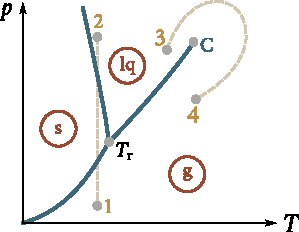
\includegraphics[scale=1]{figures/ch_15/fig_15_17.pdf}
			\caption[]{}
			\label{fig:15_17}
		\end{center}
	\end{minipage}
	\hspace{-0.05cm}
	\begin{minipage}[t]{0.5\linewidth}
		\begin{center}
			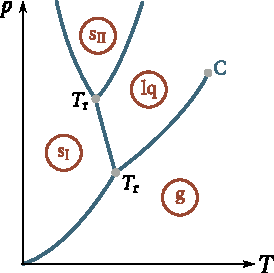
\includegraphics[scale=1]{figures/ch_15/fig_15_18.pdf}
			\caption[]{}
			\label{fig:15_18}
		\end{center}
	\end{minipage}
\end{figure}

%A phase diagram for each particular substance is plotted on the basis of experimental data. Knowing the phase diagram, we can predict the state in which a substance will be in various conditions (at various values of $p$ and $T$), and also the transformations which the substance will undergo in different processes.
Giản đồ trạng thái đối với mỗi chất cụ thể được xây dựng dựa trên những dữ liệu thực nghiệm. Biết giản đồ trạng thái, ta có thể tiên đoán chất sẽ nằm trong trạng thái nào trong những điều kiện khác nhau (với những giá trị khác nhau của $p$ và $T$), và cũng tiên đoán được cả chất sẽ bị biến đổi như thế nào trong những quá trình khác nhau.\\

%The following examples will explain this. If we take a substance in the state corresponding to point $1$ (see \fig{15_16}) and subject it to isobaric heating, then the substance will pass through the sequence of states shown by the dash straight line $1$-$2$, namely, crystals-liquid-gas. If we take the same substance in the state depicted by point $3$ and also subject it to isobaric heating, then the sequence of states (dash line $3$-$4$) will be different, namely, the crystals transform directly into a gas without passing through the liquid phase.
Ta giải thích điều đó bằng những ví dụ sau đây. Nếu ta lấy một trạng thái tương ứng với điểm $1$ trên \fig{15_16} và ta nung nóng đẳng áp nó thì chất đó sẽ đi qua một chuỗi những trạng thái biểu diễn bằng đường thẳng chấm chấm $1-2$: các tinh thể - chất lỏng - chất khí. Nếu cũng lấy chất đó ở trạng thái biểu diễn bằng điểm $3$ và cũng nung nóng đẳng áp nó thì chuỗi các trạng thái sẽ khác đi (đường thẳng chấm chấm $3-4$): các tinh thể biến trực tiếp thành khí, bỏ qua pha lỏng.\\

%It can be seen from the phase diagram that the liquid phase can exist in an equilibrium state only at pressures not lower than that of the triple point (the same relates to the solid phase II in \fig{15_18}). At pressures below $\ab{p}{tr}$ only supercooled liquids are observed. 
Từ giản đồ trạng thái ta suy ra là pha lỏng chỉ có thể tồn tại ở trạng thái cân bằng không chỉ ở các áp suất không nhỏ hơn áp suất của điểm ba (điều đó cũng đúng với pha rắn II trên \fig{15_18}). Ở những áp suất nhỏ hơn $\ab{p}{b}$, người ta chỉ quan sát thấy những chất lỏng quá lạnh.\\

%The triple point of most ordinary substances is considerably lower than atmospheric pressure. Hence, the transition of these substances from the solid state to the gaseous one occurs through the intermediate liquid phase. For instance, a pressure of \SI{4.58}{\mmHg} and a temperature of \SI{0.0075}{\degreeCelsius} correspond to the triple point of water. For carbon dioxide, the pressure at the triple point is \SI{5.11}{\atm} (the temperature of the triple point is \SI{-56.6}{\degreeCelsius}). Therefore at atmospheric pressure, carbon dioxide can exist only in the solid and the gaseous states. Solid carbon dioxide (dry ice) transforms directly into a gas. The sublimation point of carbon dioxide at atmospheric pressure is \SI{-78}{\degreeCelsius}.
Ở phần lớn các chất thông thường, điểm ba nằm thấp hơn áp suất khí quyển rất nhiều, do đó sự chuyển của những chất đó từ trạng thái lỏng sang trạng thái khí được thực hiện thông qua pha lỏng trung gian. Chẳng hạn, điểm ba của nước ứng với áp suất \SI{4.58}{\mmHg} và nhiệt độ \SI{0.0075}{\degreeCelsius}. Đối với cacbonic áp suất của điểm ba bằng \SI{5.11}{\atm} (nhiệt độ của điểm ba \SI{-56.6}{\degreeCelsius}). Vì vậy ở áp suất khí quyển cacbonic chỉ có thể tồn tại ở các trạng thái rắn và khí. Cacbonic rắn (đá khô) biến đổi trực tiếp thành khí. Nhiệt độ thăng hoa của cacbonic ở áp suất khí quyển bằng \SI{-78}{\degreeCelsius}.\\

%If the specific volume of crystals exceeds the specific volume of the liquid phase, then the behaviour of the relevant substance in some processes may be quite peculiar. Let us take, for example, such a substance in the state depicted by point $1$ (see \fig{15_17}), and subject it to isothermal compression. The pressure grows in this case, and the process is depicted in the diagram by a vertical straight line (see dash line $1$-$2$). In the course of the process, the substance passes through the following sequence of states: gas-crystals-liquid. Such a sequence is evidently observed at temperatures below that of the triple point.
Nếu thể tích riêng của các tinh thể lớn hơn thể tích riêng của pha lỏng thì hành trạng của chất đó trong một vài quá trình có thể rất là đặc sắc. Chẳng hạn, ta hãy lấy một chất như vậy ở trạng thái biểu diễn bằng điểm $1$ trên \fig{15_17} và ta nén đẳng nhiệt nó. Khi nén như vật thì áp suất tăng và quá trình được biểu diễn trên giản đồ bằng đường thẳng đứng (xem đường thẳng chấm chấm $1-2$). Trong quá trình đó chất này đi qua chuỗi các trạng thái như sau: khí - các tinh thể - trạng thái lỏng. Chuỗi giống như thế dĩ nhiên chỉ có thể quan sát được ở các nhiệt độ thấp hơn nhiệt độ của điểm ba.\\

%In concluding, we shall note another feature of a phase diagram. The vaporization curve terminates at the critical point C. Hence, a transition from the region of liquid states to that of gaseous states is possible around the critical point without intersecting the vaporization curve (see transition $3$-$4$ in \fig{15_17} depicted by the dash curve). Figure~\ref{fig:15_11} shows how such a transition looks in a $p$-$V$ diagram. In this case, the transition from the liquid state to the gaseous one (and vice versa) is performed continuously through a sequence of one-phase states. It must be noted that the entire horizontal portion of the relevant isotherm in \fig{15_11} corresponds to the point with the coordinate $T$ taken on the vaporization curve.
Để kết luận, ta hãy nhận xét thêm một đặc điểm nữa của giản đồ trạng thái. Đường cong bay hơi chấm dứt ở điểm tới hạn $K$. Vì vậy có thể có sự chuyển từ miền các trạng thái lỏng sang miền các trạng thái khí, thực hiện theo một con đường vòng quanh điểm tới hạn mà không cắt đường cong bay hơi (xem sự chuyển $3-4$ biểu diễn bằng đường chấm chấm trên \fig{15_17}). Trên \fig{15_11} ta đã chỉ rõ sự chuyển đó được thực hiện như thế noà trên giản đồ ($p,V$). Trong trường hợp này sự chuyển từ trạng thái lỏng sang trạng thái khí (và ngược lại) được thực hiện liên tục thông qua một chuỗi các trạng thái đơn pha. Chú ý rằng một điểm có tọa độ $T$ lấy trên đường cong bay hơi ứng với toàn bộ đoạn thẳng nằm ngang của đường đẳng nhiệt tương ứng trên \fig{15_11}.\\

%The continuous transition between the liquid and the gaseous states is possible because the difference between them is more of a quantitative than of a qualitative nature. In particular, anisotropy is absent in both these states. A continuous transition from the crystalline state to the liquid or gaseous one is impossible because we know that the crystalline state is featured by anisotropy. A transition from a state with anisotropy to one without it can be performed, however, only in a jump. Anisotropy cannot be present only partly either it is present or it is absent, and there is no third possibility. This is why the sublimation and the melting curves cannot terminate at the critical point like the vaporization curve does. The sublimation curve terminates at the point $p=0$ and $T=0$, and the melting curve extends to infinity.
Sự chuyển liên tục giữa trạng thái lỏng và trạng thái khí có khả năng xảy ra, vì sự khác nhau giữa chúng mang tính chất định lượng nhiều hơn là định tính; đặc biệt, ở trong cả hai trạng thái đó đều không có tính dị hương. Sự chuyển liên tục từ trạng thái kết tinh sang trạng thái lỏng hoặc khí là không thể có được, bởi vig, như ta biết, nét đặc trưng của trạng thái kết tinh là tính dị hướng. Sự chuyển từ trạng thái có tính dị hướng sang trạng thái không có tính dị hướng chỉ có thể thực hiện được bằng một bước nhảy nghĩa là tính dị hướng không thể nào chỉ có một phần, hoặc có tính dị hướng, hoặc không có tính dị hướng, không thể có khả năng thứ ba. Vì lý do đó, đường cong thăng hoa và đường cong nóng chảy không thể bị cắt đứt giống như đường cong bay hơi bị cắt đứt ở điểm tới hạn. Đường cong thăng hoa đi đến điểm $p=0$ và $T=0$, đường cong nóng chảy đi ra vô cực.\\

%In exactly the same way, a continuous transition from one crystalline modification to another is impossible. Different crystalline modifications of a substance differ in their inherent elements of symmetry. Since a symmetry element may only be either present or absent, the transition from one solid phase to another is possible only in a jump. For this reason, the equilibrium curve of two solid phases, like the melting curve, extends to infinity.
Cũng đúng như thế không thể có sự chuyển liên tục từ hình thức kết tinh này sang hình thức kết tinh khác. Những hình thức kết tinh khác nhau của một chất phân biệt với nhau ở những yếu tố đối xứng đặc thù cho chúng. Vì một yếu tố đối xứng nào đó cũng chỉ có thể hoặc là có mặt, hoặc là không, nên sự chuyển từ một pha rắn sang một pha rắn khác chỉ có thể thực hiện được bằng một bước nhảy. Vì lý do đó, đường cân bằng của hai pha rắn sẽ đi ra vô cực, tương tự như đường nóng chảy.
